\documentclass[a4paper]{IEEEtran}
\IEEEoverridecommandlockouts
\usepackage[noadjust]{cite}
\usepackage{csquotes}
\usepackage[english]{babel}
\usepackage{cite}
\usepackage{hyperref}
\usepackage{amsmath,amssymb,amsfonts}
\usepackage{graphicx}
\usepackage{textcomp}
\usepackage{xcolor}
\usepackage{array}
\usepackage{tikz}
\usepackage{etoolbox}
\usepackage{url}
\usepackage[linesnumbered]{algorithm2e}

% make algorithm2e work with IEEEtran
\makeatletter
\newcommand{\removelatexerror}{\let\@latex@error\@gobble}
\makeatother

% adjust algorithm2e to IEEEtran style
\SetAlCapNameFnt{\footnotesize}
\SetAlCapFnt{\footnotesize}

% remove semicolons in algorithm env
\BeforeBeginEnvironment{algorithm}{\DontPrintSemicolon}

% group citations
\renewcommand{\citepunct}{,\penalty\citepunctpenalty\,}
\renewcommand{\citedash}{--}

% make urls work in biblatex
\def\UrlBreaks{\do\/\do-}
\apptocmd{\sloppy}{\hbadness 10000\relax}{}{}
\def\BibTeX{{\rm B\kern-.05em{\sc i\kern-.025em b}\kern-.08em
T\kern-.1667em\lower.7ex\hbox{E}\kern-.125emX}}

% not *that* bad
%\hbadness=2521
\hbadness=10000

\begin{document}

\title{Integrating Ecovisor into Mosaik Co-Simulation}

\author{Marvin Steinke and Henrik Nickel\\\textit{Technische Universität Berlin}}

\maketitle

\begin{abstract}
    To reduce emissions, cloud platforms must increasingly rely on renewable
    energy sources such as solar and wind power. Nevertheless, the issue of
    volatility associated with these sources presents a significant challenge,
    since current energy systems conceal such unreliability in hardware. Souza
    et al. have devised a solution to this issue by creating an
    \enquote{ecovisor}. This system virtualizes the energy infrastructure and
    allows for software-defined control to be accessible by applications.
\end{abstract}

\section{Introduction}
\label{sec:introduction}
The surge of cloud platforms in recent years has had a significant impact on
many businesses and individuals, offering access to innovative and valuable
applications that frequently require significant computational resources. With
% AI as prime example, OpenAI as case study?
the increasing demand for more computational power, the cloud platforms have
become an essential part of the digital landscape. These platforms allow for the
storage, processing and management of large amounts of data and computational
resources, which can be used to run applications and services that are beyond
the capabilities of traditional hardware systems.

However, while the growth of cloud platforms has brought many benefits, it has
also raised concerns about their environmental impact. As the demand for
computational resources increases, so does the carbon emissions generated by the
energy consumption of these platforms. The carbon footprint of cloud platforms
has become a major concern, as the energy consumption of these systems is
rapidly increasing, contributing to the growing problem of climate change.
Despite their environmental impact, the growth of cloud platforms shows no signs
of slowing down. To mitigate their impact on the environment, cloud platforms
are now looking for ways to reduce their carbon footprint. It is imperative to
adopt cleaner energy sources for powering data centers, both in the cloud and at
the edge.

Although clean energy offers numerous advantages, it is perceived as being
unreliable due to two key factors. Firstly, the generation of renewable energy
sources such as solar and wind is impacted by environmental variations.
Secondly, the carbon-intensity of grid power also experiences fluctuations as
the grid employs various types of generators with varying carbon emissions to
meet demand. The field of computing possesses a distinct advantage in terms of
reducing its carbon impact through the utilization of cleaner energy sources,
even with their inherent instability. However, current cloud applications are
unable to leverage these benefits to optimize their carbon efficiency. This is
because the energy system obscures the instability of clean energy with a
reliability abstraction, which gives no control or visibility into the energy
supply. As a result, applications cannot adjust their power usage in response to
changes in the availability and carbon-intensity of renewable energy.

Souza et al. proposed a solution to this issue by creating an
\enquote{Ecovisor}, which virtualises the energy system and provides
software-based control over it. This Ecovisor enables each application to manage
the instability of clean energy through software, customized to meet its unique
requirements.

% however, setting up a system with Ecovisor is expensive, time consuming, etc.
% -> simulate Ecovisor
% but we still want real applications in our Ecovisor infra
% -> *only* simulate Ecovisor
% we present our approach that makes this possible


\section{Background}
\label{sec:background}
\subsection{Co-Simulations and Mosaik}
%The use of Mosaik brings several benefits compared to traditional simulation
%methods. It offers a more flexible and scalable simulation environment, enabling
%the integration of multiple components and the simulation of large-scale
%systems. Furthermore, it offers a more accurate representation of the energy
%system, incorporating real-world data and parameters, which can be used to
%validate the performance of the Ecovisor.
\subsection{Ecovisor}


\section{Related Work}
\label{sec:related_work}
In research and development processes, the utilization of physical testbeds is a
widespread practice \cite{cintuglu2017, mambretti2015}. They serve as a medium
for testing and evaluating new technologies, systems, and products prior to
their market launch or further development. However, some scenarios and
conditions may not be feasible or safe to recreate in a physical testbed.
Simulations can provide a controlled and cost-effective environment for testing
such scenarios and conditions \cite{mansouri2020}. When specific physical or
software components require a certain degree of realism though, simulations or
co-simulations with SIL or HIL methodologies can effectively address these
limitations.

For instance, Beilharz et al. \cite{beilharz2021}, introduce Marvis, a framework
that provides a comprehensive staging environment for testing distributed IoT
applications. Marvis orchestrates hybrid testbeds, co-simulated domain
environments, and a central network simulation to create a representative
operating environment for the system. However, Marvis does not provide a
virtualized energy system, which is crucial to meet the requirements of our
problem statement.

Hagenmeyer et al. \cite{hagenmeyer2016} investigate the interplay of different
forms of energy on various value chains in Energy Lab 2.0. The focus is on
finding novel concepts to stabilize the volatile energy supply of renewables
through the use of storage systems and the application of information and
communication technology tools and algorithms. The smart energy system
simulation and control center is a key element of Energy Lab 2.0 and consists of
three parts: a power-hardware-in-the-loop experimental field, an energy grid
simulation and analysis laboratory, and a control, monitoring, and visualization
center. While this smart energy system simulation is similar to the simulated
Ecovisor in our approach, the control center is the only entity with
software-based control over this energy system. The Ecovisor infrastructure,
however, provides multiple applications with the ability to manage their energy
supply themselves which is an essential factor for our approach.

In conclusion, to the best of our knowledge, there is no current approach that
can simulate an energy system virtualizer with software-based control,
comparable to the Ecovisor, with SIL capabilities.


\section{Approach}
\label{sec:approach}
% outline overall design with figure from pres
% intro subsections

\begin{figure}
    \centering
    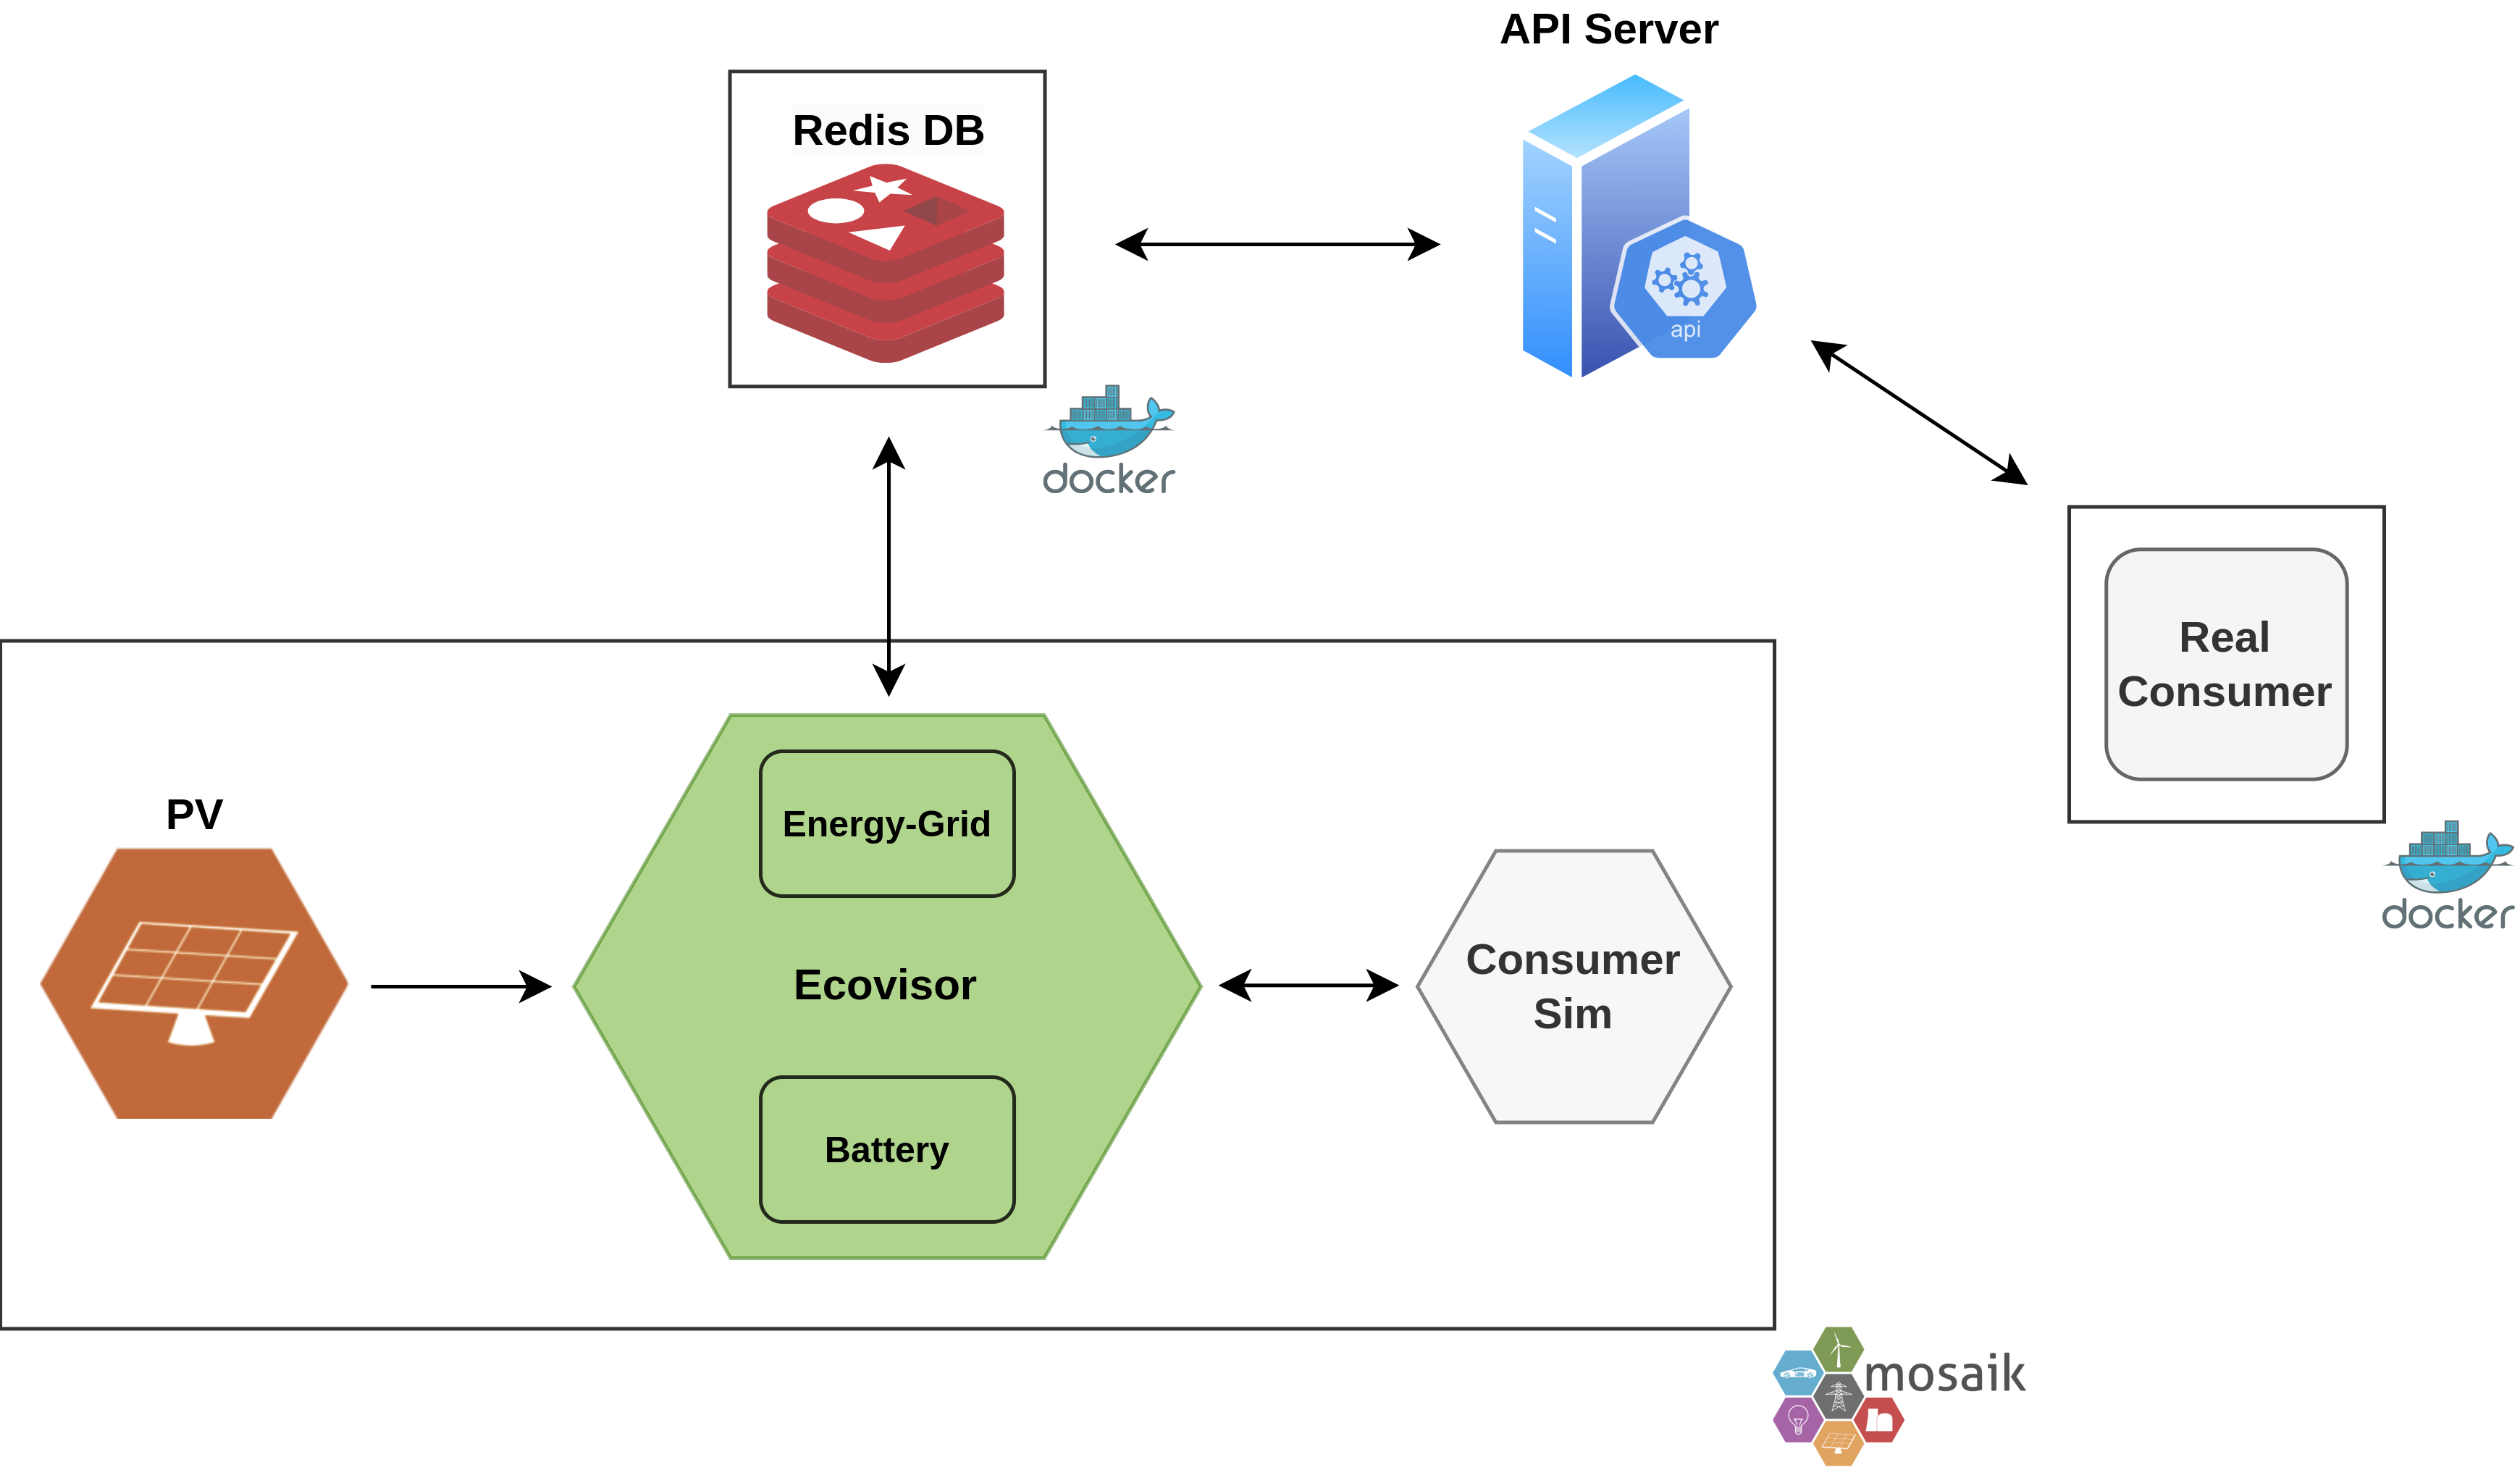
\includegraphics[width=\linewidth]{figures/system_design}
    \caption{System Design}
    \label{fig:system_design}
\end{figure}

\subsection{Simulation of the Ecovisor}

\subsection{Interface to External Applications}
ToDo: Second itteration on writing

For connecting the Ecovisor-Model to a real workload, we had to expose the API described in \cite{souza2023}. We have tried to implement it as it would probably be implemented in a real cloud environment. %source?
To achive that, we implemented the API of the Ecoviser with a RedisDB as value store between the ecovisor and the api-server. This also ensures atomiticity on the writes of the values. %sourec

The API integration itself cosists of three parts, the API-Server, the RedisDB and the Ecovisor-Redis-Interface
%Picture API
%\begin{figure}
%    \centering
%    \includegraphics[width=\linewidth]{}
%    \caption{Ecovisor API}
%    \label{fig:ecovisor_api}
%\end{figure}



\subsubsection{API-Server}
The API Server exposes the Ecoviser-APi to the "Workloads". It is implemented with the FastAPI Framework and Utilizes Uviorn to handel multiple clients accessing the API.
The Module is started as aan independent thread. In earlyer versions we tried to implement it inside of the ecovisor model, but due to the way uvicorn starts the API-Server,
it would stops the execution of the simulation until the API-Server is stopped and so we decided to design it as a standalone module. This als enables the API-Server to be scaled indipendetn from
the Ecovisor-Model and the RedisDB. This may be helpful in bigger simulations with distributed infrastructur. 


\subsubsection{RedisDB}
The RedisDB is used to interchange the values provided by eiterh ecovisor or the workload application. The database itself is a fast in memory key value store, wich is started as a docker container via the docker python libary %quelle pyton lib
to keep manual managment of the simulation to a minimum.

In general the Database can be exchanged with any other database by adapting the Ecovisor-Redis-Interface in the Ecovisor model. This can be useful when simulation should be integrated 
in a production grade cloud environment like kubernetes or open stack.

%values picture

\subsubsection{Ecovisor-Redis-Interface}


\subsubsection{Dataflow}
%Picture Data-Flow (Values set by Ecovisor, Values set by Workload)
%\begin{figure}
%    \centering
%    \includegraphics[width=\linewidth]{}
%    \caption{Dataflow betwen Ecovisor and API Server}
%    \label{fig:ecovisor_api}
%\end{figure}



\section{Evaluation}
\label{sec:evaluation}
To assess the effectiveness of our system, we conducted a two-part evaluation using open-source real-world data. We designed two example cases to demonstrate the simulation capabilities of Ecovisor and showcase how the implemented API can be used by consumers. To improve the clarity of the data presented in our examples, we scaled down the Photo Voltaic (PV) data to approximately 30\% of its original values. This allowed us to better showcase the API usage and plotted graphs. Scaling down the input data did not impact the simulation itself, as we could simply assume that less solar power was available due to weather or limitations of the solar power generators.

In the first part of our evaluation, we demonstrate the general functionality of the Ecovisor model and showcased how the output changed with varying input of the energy mix.\\
 In the second example, we highlighted a missing functionality of the API by demonstrating how a workload application can set the \textit{battery\_charge\_rate} and \textit{battery\_max\_discharge}.
 
To enhance the comprehensibility of our evaluation, we included two plots visualizing the output data from the simulation. One plot was included for each example, helping to clearly illustrate the results of our evaluation.

%To evaluate the functionality of our system, we designed two example-cases to show, how the simulation of the Ecovisor works and how the implemented API is used by a consumer. For this we used open source real world data.
%To fit the data into our examples, we scaled the Photo Voltaic (PV) Data down to ~30\% of its original values. This enhances the visibility fo the API usage and the data in the plotted graphs. Scaling down the input data does not affect the simulation itself, since we can just assume, that less solar power is available due to weather or limitations of the solar power generators.\\
%We divided our showcases into two parts, the first one showing the general functionality of the Ecovisor model and how the output changes with different changing input of the energy mix.\\
%The second example shows the missing functionality of the API, which is used by a workload application to set the \textit{battery\_charge\_rate} and the \textit{battery\_max\_discharge}.

\subsection{Ecovisor-Model with changing energy input}

\begin{figure*}
	\centering
	\begin{tikzpicture}
		\begin{axis}[
			xlabel={Time in s},
			ylabel={Energy in kWs},
			ymajorgrids=true,
			grid style=dashed,
			legend pos=outer north east,
			]
			
			\addplot[color=red, mark=dot]
			table [x=time, y=consumption, col sep=comma]
			{figures/scenario_b.csv};
			\addlegendentry{Consumption}
			
			\addplot[color=yellow, mark=dot]
			table [x=time, y=solar_power, col sep=comma]
			{figures/scenario_b.csv};
			\addlegendentry{PV Power}
			
			\addplot[color=gray, mark=dot]
			table [x=time, y=grid_power, col sep=comma]
			{figures/scenario_b.csv};
			\addlegendentry{Grid Power}
			
			\addplot[color=blue,mark=dot]
			table[x=time, y=battery_charge_level, col sep=comma]
			{figures/scenario_b.csv};
			\addlegendentry{Battery Charge Level}
			
		\end{axis}
	\end{tikzpicture}
	\caption{Showcase changing Energy Mix}
	\label{fig:example_case_a}
\end{figure*}



The first example showcased the general functionality of the Ecovisor model and how the output is affected by changing availability of different energy sources. For this simulation, we utilized an example carbon data to determine the amount of carbon emitted when using grid energy and a solar energy input file, which was scaled down to one-third of its original value. Starting from second 200, we further scaled it down until the output was under the total consumption of the workload application. In addition, we set the \textit{battery capacity} to 0.3 KW/h and the \textit{battery\_charge\_level} to 0.15 KW/h.

In the plot \ref{fig:example_case_a}, we can observe that the \textit{Grid Power} output is opposite to the PV Power output until second 200. This is because when enough PV energy is available, the surplus energy is fed into the energy grid, resulting in negative carbon emission. During the first 200 seconds, the workload application's consumption is stable at 500 KWs and doesn't change throughout the simulation. Although this isn't ideal in a real-world scenario, it allowed us to more easily demonstrate the functionality of the model.

In the first third of the simulation, until second 100, we can see that there is enough PV energy to run the workload and feed some extra energy into the grid. However, the Battery Charge Level isn't high enough to load the battery consistently. Around second 100, the PV Energy level rises, and the battery starts charging until second 200. At second 200, the PV Energy level drops, and the workload application uses the energy in the battery and from the available PV energy to meet its demands. Around second 350, no PV Energy is available, and the workload only runs on grid power until the end of the simulation. The battery doesn't charge since it only charges with PV energy.

This example demonstrates how the Ecovisor model behaves with different available energy sources. It charges the battery when enough PV energy is available and uses all other available energy before utilizing grid energy to reduce carbon emission.


\subsection{Additional API Functionality}

\begin{figure*}
	\centering
	\begin{tikzpicture}
		\begin{axis}[
			xlabel={Time in s},
			ylabel={Energy in kWs},
			ymajorgrids=true,
			grid style=dashed,
			legend pos=outer north east,
			]
			
			\addplot[color=red, mark=dot]
			table [x=time, y=consumption, col sep=comma]
			{figures/scenario_a.csv};
			\addlegendentry{Consumption}
			
			\addplot[color=yellow, mark=dot]
			table [x=time, y=solar_power, col sep=comma]
			{figures/scenario_a.csv};
			\addlegendentry{PV Power}
			
			\addplot[color=gray, mark=dot]
			table [x=time, y=grid_power, col sep=comma]
			{figures/scenario_a.csv};
			\addlegendentry{Grid Power}
			
			\addplot[color=blue,mark=dot]
			table[x=time, y=battery_charge_level, col sep=comma]
			{figures/scenario_a.csv};
			\addlegendentry{Battery Charge Level}
			
		\end{axis}
	\end{tikzpicture}
	\caption{Showcase additional API Functionality}
	\label{fig:example_case_b}
\end{figure*}

The second showcase, illustrated in Figure \ref{fig:example_case_b}, employs the same PV and Carbon data as in the first showcase, resulting in the same correlation between PV Energy and Grid Energy. The objective of this showcase is to demonstrate the usage of the API endpoints for setting the \textit{container\_powercap}, the \textit{battery\_charge\_rate}, and the \textit{battery\_max\_discharge}.

While the \textit{container\_powercap} was also utilized in the first showcase, the consumption set in the beginning remained constant. In this showcase, we developed a Python script that emulates a workload application by sending API requests to adjust the \textit{container\_powercap} around second 45 from 500 KWs to 250 KWs, which is clearly discernible in the plot. This capability enables a workload application to dynamically adjust its power consumption while scaling up or down.

Furthermore, the \textit{battery\_charge\_rate} and \textit{battery\_max\_discharge} are utilized to operate the battery. The \textit{battery\_charge\_rate} determines how much of the available PV Energy is used to charge the battery, while the \textit{battery\_max\_discharge} sets the threshold of energy that will not be used. These parameters can be adjusted to either extend the battery's lifespan or to implement different energy usage profiles. We changed both values by sending API requests with the same Python script used to set the \textit{container\_powercap}. At around second 75, we can observe that after setting both battery control values to 10 KWs, the battery begins to charge even when the available energy does not change.

\section{Future Work}
\label{sec:future_work}
While our approach focused on a single simulation of the ecovisor, our use of
Mosaik demonstrates its effectiveness for large-scale smart grid simulations. In
future research, we suggest interconnecting multiple ecovisor systems to share
resources and further reduce carbon emissions. This network could be distributed
across different geographic regions, as carbon intensity varies depending on
location. By incorporating carbon information services like Electricity Maps
\cite{electricity_maps}, this could enable carbon-efficiency optimizations such
as Let’s Wait Awhile \cite{wiesner2021} or Cucumber \cite{wiesner2022} from
Wiesner et al. This would enhance the potential for carbon reduction at a larger
scale.


\section{Conclusion}
\label{sec:conclusion}
In this article, we simulated Souza et al.'s \cite{souza2023} ecovisor and
integrated it into a Mosaik co-simulation. This design abstracts the physical
implementation and allows for the interaction with various simulators, such as
simulated virtual energy resources or simulated consumers. To integrate real
applications into this environment, we have enabled SIL and HIL capabilities by
exposing the ecovisor API through a FastAPI server that is connected to a Redis
database. We have devised a cost-effective and time-efficient approach for
testing and developing carbon-aware applications that does not require a
physical ecovisor implementation. In order to assess our approach, we generated
test cases by utilizing recorded solar and carbon data. These tests aimed to
showcase the ecovisor model's implementation accuracy and its capability to
transfer data correctly between the model and other systems.


\bibliographystyle{IEEEtran}
\bibliography{refs}

\end{document}
